% 标单百分号的注释,如本句所示。是原本模板注释
%%% 标三个百分号的注释,如本句所示。是辅助使用者理解的指导性演示,以“-BEGIN”与“-END”进行标记代码的起始位置和结束位置

%%% 与此同时,本文档作为包含子文件与分页符演示,其余功能演示内容详见 ./section/2.3.1_步兵机器人.tex 文档

% 引入导言区配置文件

%%% 包含子文件演示-BEGIN
% 文档全局设定与引入必要宏包

\documentclass[a4paper, twoside, zihao=-4, sub3section]{article}
\usepackage[hmargin=0.79in, top=0.95in, bottom=1.13in]{geometry}
\geometry{headsep=0.14in, footskip=0.47in}

\usepackage{pdfpages}
\usepackage{amsmath}
\numberwithin{figure}{section}
\usepackage{fancyhdr}

\usepackage{graphicx}
\usepackage{float}

\usepackage{ltxtable}
\usepackage{colortbl}
\usepackage{multirow}
\usepackage{graphicx}

% 字体配置

\usepackage[UTF8, heading=true]{ctex}
\setmainfont{Arial}
\setsansfont{Arial}
\setCJKmainfont[AutoFakeBold, AutoFakeSlant]{SimSun.ttc}
\setCJKsansfont[AutoFakeBold, AutoFakeSlant]{SimHei.ttf}

% 段落格式配置

\linespread{1.62}
\setlength{\parskip}{5pt}

% 目录配置

\usepackage[titles]{tocloft}
\usepackage{hyperref}
% 去除引用红框,改变颜色
\hypersetup{colorlinks=true,linkcolor=black}
% 重新定义目录的标题样式
\renewcommand*\contentsname{\hfill \color{black}\zihao{-2}\textbf{目录} \hfill}
% 设置点间距
\renewcommand\cftdotsep{0.1}
\renewcommand\cftsecdotsep{\cftdotsep}
\CTEXsetup[name={,.}]{section}
% 调节缩进
\setlength{\cftsubsecindent}{1em}
\setlength{\cftsubsubsecindent}{3em}
% 调节编号宽度
\setlength{\cftsecnumwidth}{14pt}
\setlength{\cftsubsecnumwidth}{20pt}
\setlength{\cftsubsubsecnumwidth}{30pt}
% 调节行距
\setlength{\cftbeforesecskip}{0pt}

% 标题配置

\usepackage{xcolor}
\newcommand{\titlecolor}{\color[RGB]{51, 51, 153}}
\usepackage{titlesec}
\titleformat{\section}
  {\titlecolor\zihao{2}\bfseries}
  {\thesection.}{0.5em}{}
\titleformat{\subsection}
  {\titlecolor\zihao{-2}\bfseries}
  {\thesubsection}{0.5em}{}
\titleformat{\subsubsection}
  {\titlecolor\zihao{3}\bfseries}
  {\thesubsubsection}{0.5em}{}
% 四级标题
\setcounter{secnumdepth}{4}
\titleformat{\paragraph}
  {\titlecolor\zihao{-3}\bfseries}
  {\theparagraph}{0.5em}{}

% 表格样式配置

\definecolor{tabhdcolor}{hsb}{0, 0, 0.72353}
\definecolor{gndcolor}{hsb}{0, 0, 0.96}
\AtBeginEnvironment{longtable}{\sffamily}
\renewcommand{\arraystretch}{1.1}
%%% 包含子文件演示-END
%%% 包含子文件,相当于把被包含的文件全部内容复制粘贴到此处

% 文档内容-BEGIN
\begin{document}

    % 引入封面
    % 封面

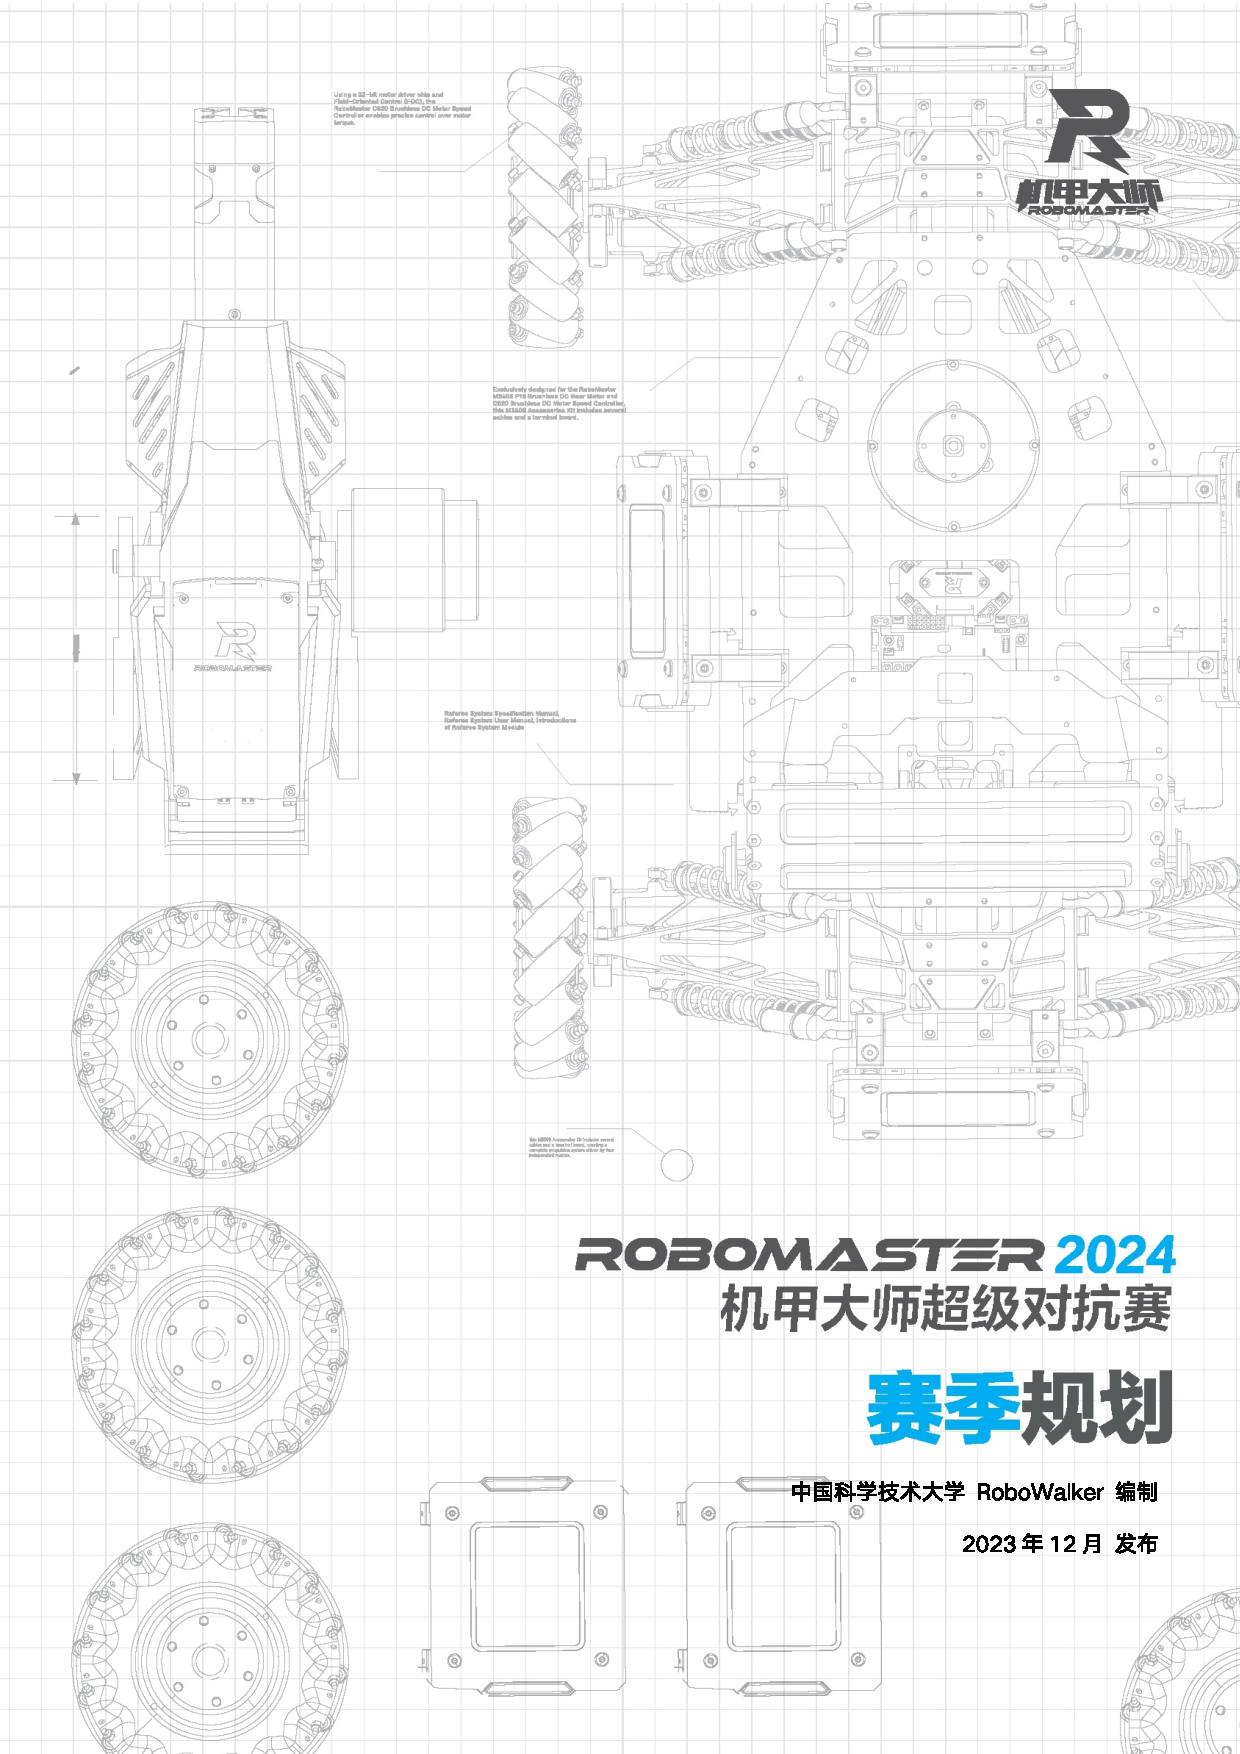
\includepdf{section/cover1.pdf}

% 编码页数从1开始
\setcounter{page}{1}

% 页眉页脚
\pagestyle{fancy}
\fancyhf{}
\fancyhead[EL, OR]{
  
\includegraphics[height=0.15in]{figure/header_img.png}
}
\fancyfoot[EL]{
  \zihao{-4}\thepage
  \hspace{0.4cm}
  \raisebox{.15ex}{
    \color{gray}{
      \zihao{-5}© 2024 \ 大疆创新 \ \ 版权所有
    }
  }
}
\fancyfoot[OR]{
  \raisebox{.15ex}{
    \color{gray}{
      \zihao{-5}© 2024 \ 大疆创新 \ \ 版权所有
    }
  }
  \hspace{0.4cm}
  \zihao{-4}\thepage
}

% 目录
\begin{center}
  \zihao{5}\tableofcontents
\end{center}

\newpage
    
    \input{section/0_前言}
    
    %%% 分页符演示-BEGIN
    \newpage
    %%% 分页符演示-END
    %%% 分页符,相当于从此处开辟新的一页,无论上一页内容是否凑够一页,都会从新的一页开始
    
    \input{section/1_团队目标}
    
    \newpage
    
    \input{section/2_项目分析}
    
    \input{section/2.1_上赛季项目分析经验}
    
    \input{section/2.2_新赛季规则解读}
    
    \input{section/2.3_研发项目规划}
    
    \input{section/2.3.1_步兵机器人}
    
    \input{section/2.3.2_英雄机器人}
    
    \input{section/2.3.3_工程机器人}
    
    \input{section/2.3.4_哨兵机器人}
    
    \input{section/2.3.5_空中机器人}
    
    \input{section/2.3.6_飞镖系统}
    
    \input{section/2.3.7_雷达}
    
    \input{section/2.3.8_人机交互}
    
    \input{section/2.4_技术储备规划}
    
    \input{section/2.4.1_通用技术储备}
    
    \input{section/2.4.2_特定兵种技术储备}
    
    \newpage
    
    \input{section/3_团队架构}
    
    \newpage
    
    \input{section/4_资源可行性分析}
    
    \newpage
    
    \input{section/5_宣传及商业计划}
    
    \input{section/5.1_宣传计划}
    
    \input{section/5.2_商业计划}
    
    \newpage

    % 引入封底
    % 封底
    

\includepdf{section/cover2.pdf}

\end{document}
%%% 文档内容-END
%%% 文档内容是正文部分,我们只需编辑 ./section/ 目录下的文档即可